% The preceding line is only needed to identify funding in the first footnote. If that is unneeded, please comment it out.
\documentclass[conference]{IEEEtran}
\pagestyle{plain}
\usepackage{fontspec}
\usepackage{tikz}
\usetikzlibrary{shapes,snakes}
\usepackage{amsmath,amssymb,amsfonts}
\usepackage{algorithmic}
\usepackage{graphicx}
\usepackage{subcaption}
\usepackage{textcomp}
\usepackage{xcolor} 
\usepackage{comment}
\usepackage{booktabs}
\usepackage{multicol}
\usepackage{stfloats}
\usepackage{nameref}
\usepackage{svg}



\def\BibTeX{{\rm B\kern-.05em{\sc i\kern-.025em b}\kern-.08em
    T\kern-.1667em\lower.7ex\hbox{E}\kern-.125emX}}
\usepackage[numbers,sort&compress]{natbib}

\makeatletter
\newcommand\subparagraph{\@startsection{subparagraph}{5}{\z@}%
  {-1.25ex\@plus -1ex \@minus -.2ex}%
  {0.5ex \@plus .2ex}%
  {\normalfont\normalsize\bfseries}}
\makeatother

% Some colors
\definecolor{c1}{RGB}{84, 156, 22}
\definecolor{c2}{RGB}{190, 214, 71}
\definecolor{c3}{RGB}{212, 197, 38}
\definecolor{c4}{RGB}{212, 125, 38}
\definecolor{c5}{RGB}{194, 36, 21}
\definecolor{dottedlines}{RGB}{33, 82, 117}
\definecolor{darkgreen}{rgb}{0.0, 0.4, 0.0}

% Define the command \struct
\newcommand{\note}[1]{\textcolor{darkgreen}{#1}}

\begin{document}

\title{How Does the Level of Somatosensory Feedback Fidelity Impact Motor Learning in VR: \\a Systematic Review}

\author{\IEEEauthorblockN{Reinprecht Christian}
\IEEEauthorblockA{TU Delft, NL \\
C.T.Reinprecht@student.tudelft.nl}}

\maketitle
\thispagestyle{plain}
\pagestyle{plain}

%% REVISIT %%
\begin{abstract}
Simulations in virtual reality (VR) offer a robust platform for acquiring new skills across diverse applications. The virtual environment (VE) also facilitates the study of complex skills and user performance evaluation, enhancing our understanding of motor learning. Recent research suggests that haptic feedback in VR offers a great way to improve several aspects of motor learning, including timing, accuracy, and skill transfer. The many approaches to providing haptic feedback differ in their feedback fidelity, i. e. how realistic the interaction in VR feels. However, the effect of varying levels of feedback fidelity on motor learning remains unclear. Here, we present a systematic review, in which we evaluate the feedback fidelity of the systems described in the studies using the Haptic Feedback Fidelity Framework to create a standardized basis for comparison. We enhance the framework with a confidence score, to account for the varying quality of the involved studies, and a score for the observed impact on motor learning. Our findings indicate that abstract haptic feedback, characterized by low fidelity and limited alignment with user actions, generally resulted in negative or negligible impacts on motor learning. Representational feedback, with moderate fidelity, typically produced positive outcomes, including decreased response times and enhanced performance. High-fidelity haptic feedback showed an overall positive impact on motor learning, particularly for tasks requiring ballistic movements or high precision, or involving a third dimension. With this work, we aim to improve the understanding of how different forms of haptic feedback affect motor learning, potentially making the acquisition of new skills more effective.

\end{abstract}

\begin{IEEEkeywords}
motor learning, fidelity, virtual reality, systematic review
\end{IEEEkeywords}

%%%%% INCLUDE CHAPTERS %%%%%%
%%%%% INTRODUCTION %%%%%

\section{Introduction}
The virtual environment (VE) provides a comprehensive platform for users to acquire new skills and competencies, with applications ranging from physical therapy and rehabilitation to sports and industrial training, education, marketing, telerobotics, and research, as well as gaming and entertainment \cite{Wu2023TrainingReality, Oagaz2022PerformanceReality}. 
Furthermore, simulations in virtual reality (VR) enable researchers to study complex skills and assess the motor performance of users without giving up on experimental control. This approach facilitates the understanding of motor learning on a level that is not possible in the physical world \cite{Harris2021ExploringSimulator, Levac2019LearningReview}. 
Therefore it is not surprising that there is a great interest in VR-based training simulations, especially to teach skills that would otherwise have to be acquired in dangerous or sensitive environments, such as construction work, military training, or surgical operations \cite{Adami2021EffectivenessTeleoperation, Lele2013VirtualUtility, Qi2021VirtualScenario}.

During these physical interactions in the real world, for example, when learning how to operate a knee, we rely not only on visual feedback but also on information obtained through the mechanoreceptors in our skin, and proprioceptors in our tendons, joints, and muscles \cite{Gonzalez-Grandon2021ProprioceptionInteraction}. To provide these stimuli in the virtual world, tools or devices are required to reproduce the sensations we would expect when interacting with objects in the VE, which includes the perception of pressure, vibration, temperature, and the position and movement of body parts. Exposing the user to these sensations when they are interacting with objects in VR---generally denoted as somatosensory feedback---may offer a promising approach to increase the effectiveness of motor learning \cite{Sigrist2013AugmentedReview}. 
The degree to which the feedback in the VE mimics real-world interaction is determined by its fidelity \cite{Caird1996PersistentTraining}, which ranges from simple, binary cues such as a clicking sensation to high-fidelity feedback that feels as if the user is interacting with a real object \cite{Yang2023}.

% Added reviews, the second round of going to research gap
Many studies have explored the effect of \textit{augmented haptic feedback} and \textit{haptic guidance} on motor learning, which involves guiding the user through a movement. It has shown to be beneficial for initial learning, as it decreases the error and task completion time during training \cite{Caccianiga2021, LeeH2014, Fehlberg2012}, however, it can lead to overreliance, which may result in worsened long-term retention performance \cite{Oquendo2024}. 

In contrast, for \textit{haptic rendering}---which focuses on replicating the natural haptic sensations expected when interacting with virtual environments (VEs)---it remains unclear how varying levels of feedback fidelity influence motor learning.
While researchers previously assumed that higher fidelity correlates with better training performance in VR \cite{Caird1996PersistentTraining, Waller1998TheTraining}, as the interaction feels more natural, recent research suggests that there might be no linear correlation between the level of feedback fidelity and motor performance: Instead, motor performance decreased in conditions that yielded feedback with medium feedback fidelity, compared to scenarios with high and well-designed low feedback fidelity \cite{MahdiNabiyouni201520153DUI.}.

Since supplying high fidelity to a VE is very costly, it is important to determine under which circumstances low-fidelity feedback, such as somatosensory cues, is sufficient to increase the effectiveness of motor learning, and where high-fidelity feedback is necessary. 

In this work, we therefore systematically review current research to create an overview of the impact of different levels of somatosensory feedback fidelity on motor learning in VR. To create a common ground, we first evaluate each haptic feedback system in the studies utilizing the Haptic Fidelity Framework by Muender et al. \cite{Muender2022HapticReality}. We extend the framework by a confidence score, which stands for the quality of the paper, and evaluate the found impact on motor learning in the experiments. Then, we cluster the data and address similarities and differences in the studies, and how these influence the impact of the provided haptic feedback on motor learning. 

%%%%% METHODS %%%%%

\begin{figure*}[htbp]
    \centering
    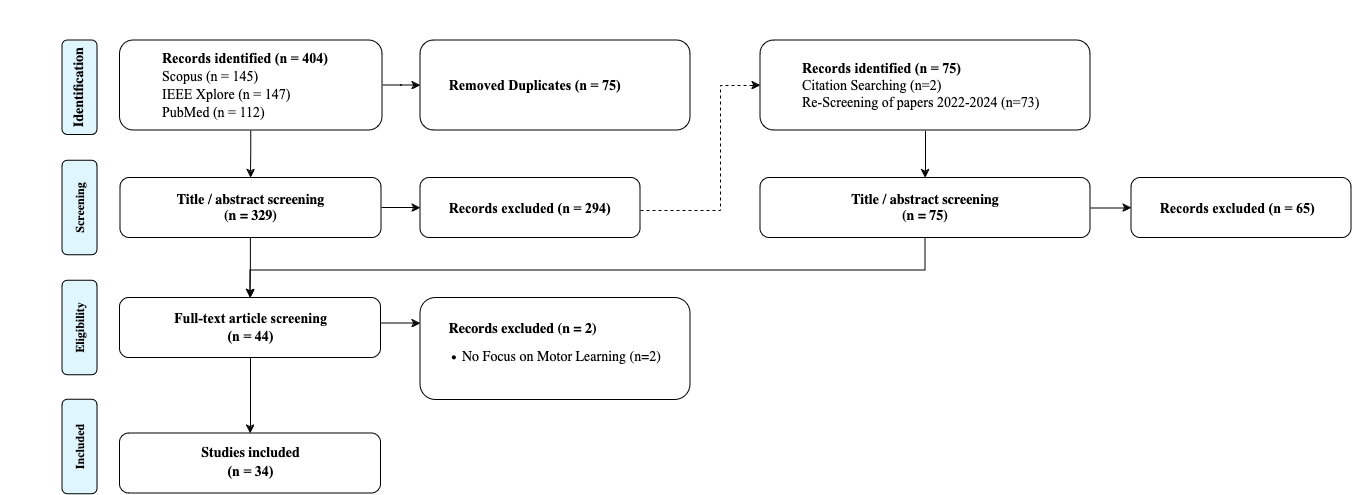
\includegraphics[width=\linewidth]{figures/prisma_overview.png} 
    \caption{Overview of the methodology using the PRISMA method}
    \label{fig:prisma}
\end{figure*} 

\section{Methods}
\label{sec:methods}

The method of the systematic review was based on the PRISMA methodology \cite{Page2021TheReviews} to ensure transparent and complete reporting on the topics examined.

\subsection{Search Strategy and Eligibility Criteria}
\label{sec:eligibility}
Several relevant articles were reviewed at the beginning to find eligible search terms. The query based on the research question consists of three main parts, namely \textit{virtual reality}, \textit{somatosensory feedback}, and \textit{motor learning}, each term with their respective synonyms. 

The final search query was as follows: motor AND (learning OR control OR training OR skills) AND (((virtual OR augmented) AND reality) OR ((remote OR virtual OR simulated) AND environment)) AND (((somatosensory OR haptic OR tactile OR proprioceptive OR kinesthetic OR cutaneous OR somatic) AND 
(cue* OR feedback OR rendering OR stimul*)) AND (fidelity OR realism OR accuracy OR precision OR exactness OR specificity)). The search terms were applied for the article title, abstract, and keywords.

Three databases (Scopus, IEEE Xplore, and PubMed) were searched in April 2024. Based on the required syntax of each database, the search query was slightly adapted. For example, as PubMed only allows for the use of an asterisk for words containing more than three letters, the term \textit{cue*} was changed to (\textit{cue} OR \textit{cues}). The exact search queries can be found in \ref{sec:queries}. 

To qualify for inclusion, studies had to focus on the impact of somatosensory feedback on motor learning in humans. We included studies with healthy participants only, as patients often know how to perform a movement but are physically constrained by their condition, therefore augmented feedback may help the motor learning of patients in a different way compared to healthy subjects \cite{Sigrist2013AugmentedReview}. There were no publication date or language limits.

Conversely, studies were excluded if they (i) did not relate to motor learning in humans; (ii) focused on systems not providing haptic feedback in VR; (iii) were concerned with a neurological condition affecting motor learning; or (iv) explained a new assessment system for the evaluation of motor learning.

\subsection{Study Selection}
At first, duplicate publications were identified and removed. The results were then screened based on their title and abstract. 

In this review, we wanted to emphasize more recent studies to reflect the significant impact of recent technological advances in VR on the field. Therefore, records published in the years 2022-2024 were re-screened and also included in the further process, if they were only partially fitting the eligibility criteria. Additional papers were identified using citation searching.

Finally, the full-text articles were assessed to determine their eligibility for inclusion in the review (see fig. \ref{fig:prisma}).


\section{Search Results}

%%%% Rewrite for precise numbers!! %%%%%

The search yielded a total of 404 results, which were saved in the library of Mendeley. 75 duplicates were found and removed. The remaining 329 records were screened based on title and abstract first. This led to the preliminary exclusion of 294 records, of which 73 records were re-screened as they were from the years 2022-2024 (see fig. \ref{fig:prisma}). 
Additionally, 2 papers were included based on citation search. 

In total, 44 articles were full-text screened. Out of these, 7 were excluded based on the exclusion criteria described in \ref{sec:eligibility}, and the remaining 34 studies were included in this review.


\subsection{Study characteristics}

\subsubsection{Year of publication}
The year of publication of the included studies ranges from 2000 to 2024. As seen in \ref{fig:years}, the number of studies has greatly increased in the past decade, with a peak in 2018.

\begin{figure}[htbp]
    \centering
    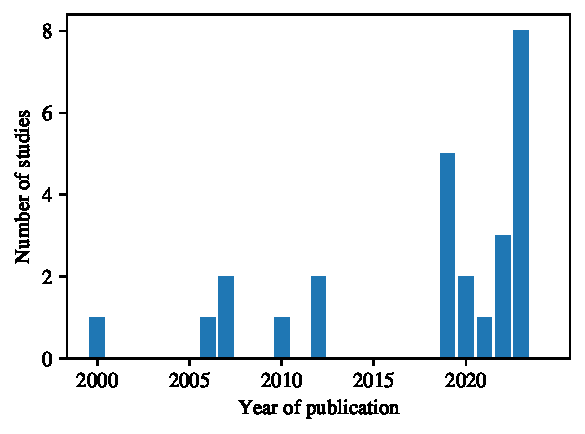
\includegraphics[width=\columnwidth]{figures/years.pdf} 
    \caption{Publication dates of the included articles}
    \label{fig:years}
\end{figure} 

\subsubsection{\struct{Body parts involved}}
Make graph to quantify which body parts are involved in which paper (make pie chart).


\section{Definitions}
\subsection{\struct{Feedback Fidelity}}
Feedback fidelity refers to the accuracy and realism of stimuli provided to the user when they are interacting with the virtual environment. 

Several frameworks have been proposed to assess the feedback fidelity of the VE. They concentrate on either the physical attributes of the system (e.g. the FIFA framework developed by McMahan et al. \cite{McMahan2011ExploringGames}), aim to evaluate feedback fidelity through questionnaires (e. g. the haptics addition \cite{Boos2017ErweiterungHaptik} to the User Experience Questionnaire \cite{Laugwitz2008ConstructionQuestionnaire}), or focus on the effect of the system. Huang et al. for example suggested that skill transfer might be a useful paradigm to evaluate the level of fidelity, assuming that if an environment has infinite fidelity and is therefore perfectly recreating the sensations of the real environment, then there would be no performance loss when transferring the skill from the virtual to the real environment \cite{Huang2006}.

These frameworks, while addressing particular subjective and objective dimensions of haptic feedback systems, fail to capture their full diversity. This gap is addressed by Muender et al., who developed the Haptic Feedback Fidelity Framework \cite{Muender2022HapticReality}.
It helps to evaluate a system's haptic feedback fidelity ranging from abstract to realistic, and introduces versatility as a second axis, which allows for the differentiation between generic and specific haptic feedback systems.

In this review paper, we extend the Haptic Feedback Fidelity Framework by a third axis, taking into account a quality score for each haptic feedback system. This score determines how many of the parameters assessed in the framework have actually been provided by the researchers. Furthermore, single aspects of the framework are extended in an attempt to make the evaluation more transparent and quantifiable. 

We then evaluate the selected articles described in section \ref{sec:methods}  based on this framework.

\section{\struct{Framework}}

The framework is built on eight foundational factors, describing th features of a system and their value, and six limiting factors that negatively impact the perception. Each factor is rated on a 5-point Likert-scale (0-4).

\subsection{\struct{Haptic Fidelity}}
\subsubsection{\struct{Foundational Factors}}
\paragraph{\struct{Body Location}}
E.g. body parts involved.
\begin{comment}
"The required refresh rate to provide realistic
force feedback is commonly accepted to be at least 1,000 Hz.
However, this refresh rate is widely debated. According to
Burdea [14], a minimum refresh rate of only 300 Hz is
acceptable. Conversely, a study by Booth et al. [15] using
SensAble’s Premium 1.5 to deduce the minimum acceptable
haptic refresh rate, suggests that “a minimum acceptable
refresh rate must lie within the 550-600 Hz range.” The
necessary rate of update is dependent upon the stiffness of
the surfaces to be simulated. A stiff contact between objects is
better simulated by higher refresh rates, whereas lower
refresh rates are satisfactory for softer objects. Additional
methods can be applied to simulate touching stiffer objects
such as combining vibrations with force to the end effector to
represent the small vibrations felt upon object contact [16].
Typically, a trade-off must be made between the accuracy of
the haptics effects produced and the speed required within
the application." \cite{Coles2011TheArt}
About latency and its impacts: \cite{Gourishetti2018PassiveFeedback}.
Ballistic movements: rapid, involuntary movement which is motor programmed, and for which visual feedback is not possible \cite{Wall2000}.
\end{comment}

\paragraph{\struct{Body Area}}
E.g. body area involved. 
\paragraph{\struct{Stimuli}}
Etc.

\paragraph{\struct{Magnitude}}
Etc.

\paragraph{\struct{Sensory Integrity}}
Etc.

\paragraph{\struct{Degrees of Freedom}}
Etc.

\paragraph{\struct{Hardware Precision}}
Etc.

\paragraph{\struct{Software Precision}}
According to \cite{Coles2011TheArt}, the minimum acceptable refresh rate must lie within the 550-600 Hz range, ...

\subsubsection{\struct{Limiting Factors}}
Etc.

\paragraph{\struct{Dependency}}
Etc.

\paragraph{\struct{Distinguishability}}
Etc.

\paragraph{\struct{Hardware Latency}}
Latency of over 25ms, according to ...

\paragraph{\struct{Software Latency}}
Etc.

\paragraph{\struct{Side Effects}}
Etc.

\paragraph{\struct{Constraints}}
Etc.

\subsection{\struct{Versatility}}

\subsection{\struct{Quality score}}
In total, there were 14 parameters which needed to be evaluated for each haptic feedback system. We calculated a score based on the percentage of parameters, that were not described in the paper itself, nor could be accessed through an internet research (example, calculation etc.).
%%%%% RESULTS %%%%%%
\twocolumn

\section{Results}
Here come the results.

\begin{figure}[]
    \centering
    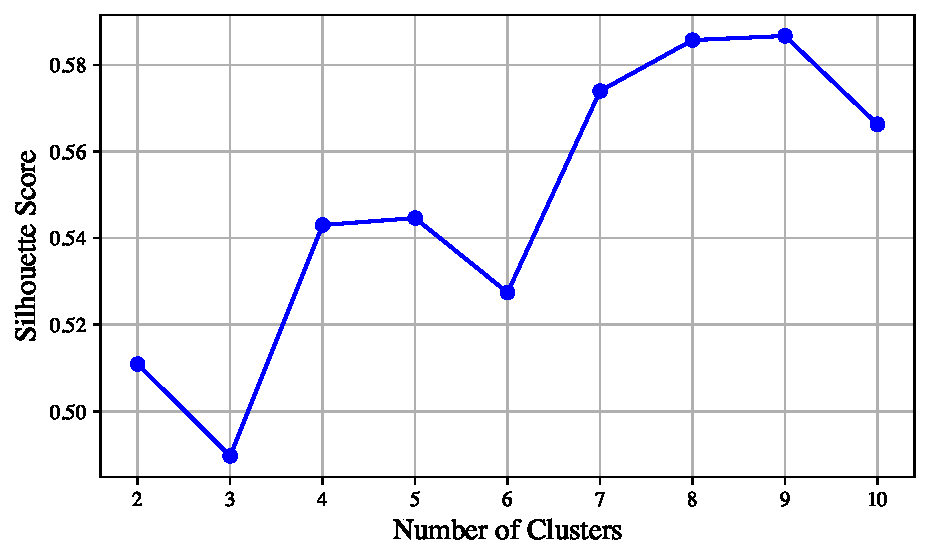
\includegraphics[width=\columnwidth]{figures/silhouette.pdf} 
    \caption{Silhouette scores for the numbers of clusters}
    \label{fig:silhouette}
\end{figure}

\begin{figure}[]
    \centering
    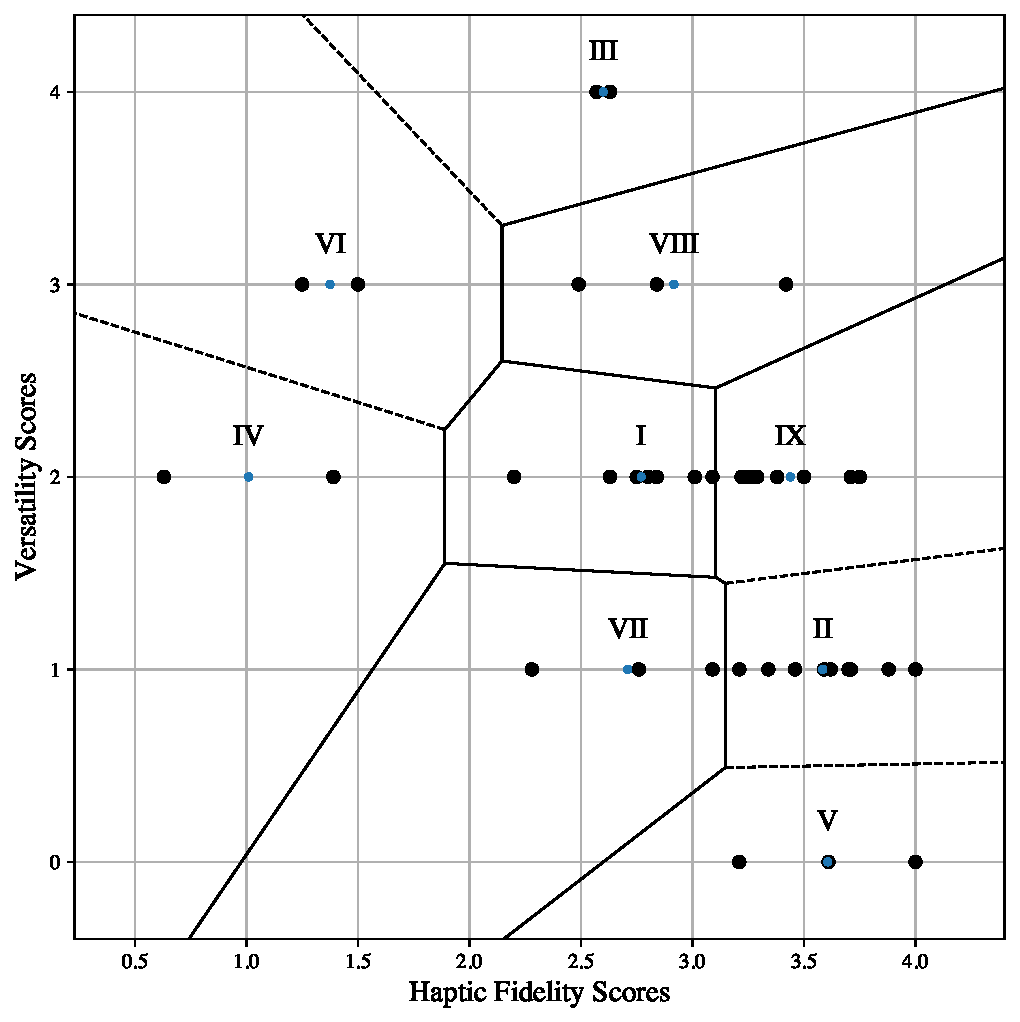
\includegraphics[width=\columnwidth]{figures/literature_data.pdf} 
    \caption{KMeans clustering of the data}
    \label{fig:kmeans}
\end{figure}





%%%%% DISCUSSION %%%%%%
\pagebreak

\section{Discussion}
% Summarize key findings of section results (\ref{sec:results}) in one or two paragraphs
% Interpretation of the results, discussion of the meaning in the context of motor learning
% Justify interpretation by citing the supporting key studies
% Discuss possible alternative interpretations of the data (if applicable)
% Mention limitations of my research 
    % Critique on framework: does not separate abstract from real tasks that are trained in the VE
    % Limitations of systematic review itself
    % Implications for future studies, mention practical implications

\paragraph{\nameref{sec:specificabstract}}
This cluster contains one paper only, in which the vibrational feedback has a negative impact on motor learning. Even though the rhythmic task itself would probably benefit from haptic feedback (as has been shown by \cite{Graham2008} in a similar task), the vibrational feedback does not match with the intended action by the user, which is a unidirectional motion. Furthermore, as described by I. Lee et al, the vibration of the drumstick itself masked the vibrational feedback at higher frequencies, which made it harder for the participants to perceive the given feedback. Furthermore, the other types of feedback (e.g. FLOW, in which flowing bars across the screen showed when to hit the drum next) allowed for an anticipation of the next movement. This creates an uneven comparison with the vibrational feedback system. Therefore, the adverse effect on motor learning caused by poorly designed low-fidelity feedback, which is further disrupted by noise within the same modality, is unsurprising.


Haptic feedback has been found to hinder motor learning, especially for tasks that naturally did not involve haptic feedback and when it was provided in a rather abstract way. Hanashima et al. for example provided vibrotactile feedback for posture learning and found the visual only condition to be superior over the visuo-tactile condition \cite{Hanashima2023}. However, when we learn a posture from another person in real life, we will also either depend on visual feedback only (for example when imitating the other person and using a mirror), or we will have actual guidance (for example from a physiotherapist). Vibrational feedback however does not seem to be a meaningful way to provide haptic feedback when learning postures.

If the haptic rendering is amplified, but pointing in the same direction (for example when amplifying the errors, \cite{Oquendo2024}), this can be especially helpful for initially better skilled subjects. However, it is worse for subjects with initially less skill, as it might be overwhelming (according to challenge point theory). If the haptic feedback is incongruent, this is always worse for motor learning. For example if the feedback is pointing in the opposite direction.

\subsection{Shortcomings of framework}
Framework mixes for haptic fidelity score multiple properties of the haptic devices and tries to accumulate these into one single score. This however does not cover the complexity of aspects that haptic devices have to offer. One example is the magnitude of feedback that is matched by the haptic device. This can either be explained by to which extent the haptic device can match the magnitude in real world, e.g. if the force in reality required 10N of force and the haptic device can render 10N of force. The other however is the force modality, as haptic devices can either render the natural forces of the object, but can also amplify the errors of the participant when doing a task, or have the forces point in the exact opposite direction. Even though this is only one in 8 evenly weighed foundational factors according to the framework \cite{Muender2022HapticReality}, it has a detrimental effect on motor learning. This is not appropriately taken into account in the framework.

\begin{comment}
Suggestions: For the post hoc evaluation of the haptic feedback fidelity, it would be helpful if researchers included specifications of the device used, such as hard- and software latency, maximum force, sensor and actuator accuracy, etc., even if the device is commercially available. This makes the objective rating of the feedback fidelity easier and quicker, as even for commercially used devices the specifications might not be available anymore at some point in the future.

Often, an artificial task is chosen, such as tracking a trajectory with a steering wheel, where the velocity of the car is constant to eliminate the use of foot pedals \cite{LeeH2014}. For the retention, the subjects are using the exact same setup, so parameters such as the degrees of freedom, and the stimuli of experiment and retention are the same, thus increasing the level of fidelity. However, the performance of the participants driving a real car, or even driving in a more realistic simulator is never evaluated, despite this actually being an interesting question. In the end, we want to know how we can effectively improve motor learning performance by providing haptic feedback to the user. If we are doing this only for artificial tasks, we are making the experimental setup easier and possibly cheaper, but not exploring the greater possibilities this technology might offer. 

One important finding is that haptic feedback might be especially important when learning a motor task that requires 3 dimensions. Studies that required the participants to follow a trajectory in 2D have often found no significant improvement in task performance when providing haptic feedback, compared to visual feedback only (\cite{Gambaro2014}, \cite{LiuG2014}, \cite{LeeH2014}), whereas studies involving trajectory following in 3 dimensions have shown a significant improvement with the introduction of haptic feedback (\cite{Grant2019}, \cite{Rodriguez2010}, ...)
    
\end{comment}


\begin{comment}
\onecolumn

\begin{tikzpicture}[scale=3.6]
    
    % Add axis labels
    \foreach \x in {0,1,2,3,4} {
        \draw [very thin, lightgray](\x cm, 0-0.05) -- (\x cm, 4+0.05) node[anchor=north] {};
        \draw [very thin, lightgray](0-0.05,\x cm) -- (4+0.05,\x cm) node[anchor=east] {};
    }

    % Draw axes
    \draw[thick,<->] (0,2) -- (4,2) node[anchor=south west] {Haptic Fidelity};
    \draw[thick,<->] (2,0) -- (2,4) node[anchor=south] {Versatility};

    \node at (0,1.9) {\footnotesize{abstract}};
    \node at (4,1.9) {\footnotesize{realistic}};
    \node at (1.8,0.1) {\footnotesize{specific}};
    \node at (1.8,3.9) {\footnotesize{generic}};

    % Legend
    \draw[fill=white] (0.1,3.9) rectangle (1.2,3.25); % Legend border
    \node[anchor=west] at (0.15, 3.8) {\textbf{Legend}}; % Legend title
    
    \node[circle, fill=c1, inner sep=2.3pt] at (0.22, 3.65) {};
    \node[anchor=west] at (0.25, 3.65) {\footnotesize{Quality $q > 0.9$}};

    \node[circle, fill=c2, inner sep=2pt] at (0.22, 3.55) {};
    \node[anchor=west] at (0.25, 3.55) {\footnotesize{Quality $0.8 < q \leq 0.9$}};

    \node[circle, fill=c3, inner sep=1.7pt] at (0.22, 3.45) {};
    \node[anchor=west] at (0.25, 3.45) {\footnotesize{Quality $0.7 < q \leq 0.8$}};

    \node[circle, fill=c4, inner sep=1.4pt] at (0.22, 3.35) {};
    \node[anchor=west] at (0.25, 3.35) {\footnotesize{Quality $q \leq 0.7$}};
    
    % Sample data points
    \node[circle, fill=c1, inner sep=2.3pt] at (3.5,2) {};
    \node[circle, fill=c1, inner sep=2.3pt] at (3.22,2) {};
    \node[circle, fill=c1, inner sep=2.3pt] at (0.63,2) {};
    \node[circle, fill=c1, inner sep=2.3pt] at (3.38,2) {};
    \node[circle, fill=c1, inner sep=2.3pt] at (3.75,2) {};
    \node[circle, fill=c1, inner sep=2.3pt] at (2.63,2) {};
    \node[circle, fill=c1, inner sep=2.3pt] at (2.75,2) {};
    \node[circle, fill=c1, inner sep=2.3pt] at (3.21,0) {};
    \node[circle, fill=c1, inner sep=2.3pt] at (4,0) {};
    \node[circle, fill=c1, inner sep=2.3pt] at (4,1) {};
    \node[circle, fill=c1, inner sep=2.3pt] at (3.88,1) {};
    \node[circle, fill=c1, inner sep=2.3pt] at (1.5,3) {};
    \node[circle, fill=c1, inner sep=2.3pt] at (3.59,1) {};
    \node[circle, fill=c1, inner sep=2.3pt] at (3.09,2) {};
    \node[circle, fill=c1, inner sep=2.3pt] at (2.57,4) {};
    \node[circle, fill=c1, inner sep=2.3pt] at (3.21,1) {};
    \node[circle, fill=c1, inner sep=2.3pt] at (3.01,2) {};
    \node[circle, fill=c1, inner sep=2.3pt] at (3.25,2) {};
    \node[circle, fill=c1, inner sep=2.3pt] at (2.84,3) {};
    \node[circle, fill=c1, inner sep=2.3pt] at (3.7,1) {};
    \node[circle, fill=c1, inner sep=2.3pt] at (2.57,4) {};
    \node[circle, fill=c1, inner sep=2.3pt] at (3.5,2) {};
    \node[circle, fill=c2, inner sep=2.0pt] at (2.63,4) {};
    \node[circle, fill=c2, inner sep=2.0pt] at (2.84,2) {};
    \node[circle, fill=c2, inner sep=2.0pt] at (3.27,2) {};
    \node[circle, fill=c2, inner sep=2.0pt] at (3.34,1) {};
    \node[circle, fill=c2, inner sep=2.0pt] at (3.46,1) {};
    \node[circle, fill=c2, inner sep=2.0pt] at (3.46,1) {};
    \node[circle, fill=c2, inner sep=2.0pt] at (3.46,1) {};
    \node[circle, fill=c2, inner sep=2.0pt] at (3.62,1) {};
    \node[circle, fill=c2, inner sep=2.0pt] at (3.75,2) {};
    \node[circle, fill=c2, inner sep=2.0pt] at (3.09,1) {};
    \node[circle, fill=c2, inner sep=2.0pt] at (3.71,1) {};
    \node[circle, fill=c2, inner sep=2.0pt] at (3.29,2) {};
    \node[circle, fill=c2, inner sep=2.0pt] at (2.28,1) {};
    \node[circle, fill=c2, inner sep=2.0pt] at (3.42,3) {};
    \node[circle, fill=c2, inner sep=2.0pt] at (2.76,1) {};
    \node[circle, fill=c2, inner sep=2.0pt] at (3.71,2) {};
    \node[circle, fill=c3, inner sep=1.7pt] at (2.2,2) {};
    \node[circle, fill=c3, inner sep=1.7pt] at (2.8,2) {};
    \node[circle, fill=c3, inner sep=1.7pt] at (1.25,3) {};
    \node[circle, fill=c3, inner sep=1.7pt] at (1.39,2) {};
    \node[circle, fill=c3, inner sep=1.7pt] at (2.49,3) {};
    \node[circle, fill=c3, inner sep=1.7pt] at (3.61,0) {};
    \node[circle, fill=c3, inner sep=1.7pt] at (1.08,1) {};
    \node[circle, fill=c3, inner sep=1.7pt] at (2.31,3) {};
    \node[circle, fill=c4, inner sep=1.4pt] at (4,1) {};


    % Add citations to datapoints
    \node at (3.5,2.1) {\footnotesize{\cite{Brickler2019}}};
    \node at (3.22,2.1) {\footnotesize{\cite{Caccianiga2021}}};
    \node at (0.63,2.1) {\footnotesize{\cite{Crespo2015}}};
    \node at (3.38,1.9) {\footnotesize{\cite{Feygin2002HapticSkill}}};
    \node at (3.75,2.2) {\footnotesize{\cite{Feygin2002HapticSkill}}};
    \node at (2.63,2.1) {\footnotesize{\cite{Gambaro2014}}};
    \node at (2.75,1.9) {\footnotesize{\cite{Gambaro2014}}};
    \node at (3.21,0.1) {\footnotesize{\cite{Graham2008}}};
    \node at (4,0.1) {\footnotesize{\cite{Huang2006}}};
    \node at (4,1.1) {\footnotesize{\cite{Huang2007}}};
    \node at (3.88,1.1) {\footnotesize{\cite{LeeH2014}}};
    \node at (1.5,3.1) {\footnotesize{\cite{LiuH2019}}};
    \node at (3.59,1.1) {\footnotesize{\cite{Mohanty2023}}};
    \node at (3.09,1.9) {\footnotesize{\cite{Oquendo2024}}};
    \node at (2.57,3.9) {\footnotesize{\cite{Vasudevan2020}}};
    \node at (3.21,1.1) {\footnotesize{\cite{Dai2023}}};
    \node at (3.01,2.1) {\footnotesize{\cite{Dai2023}}};
    \node at (3.25,1.9) {\footnotesize{\cite{Gunter2022}}};
    \node at (2.84,3.1) {\footnotesize{\cite{LeeY2019}}};
    \node at (3.7,1.1) {\footnotesize{\cite{LiuG2014}}};
    \node at (2.57,4.1) {\footnotesize{\cite{McAnally2023}}};
    \node at (3.5,2.2) {\footnotesize{\cite{Rodriguez2010}}};
    \node at (2.7,4.1) {\footnotesize{\cite{Yang2023}}};
    \node at (2.84,2.2) {\footnotesize{\cite{Yang2023}}};
    \node at (3.27,2.2) {\footnotesize{\cite{Yang2023}}};
    \node at (3.34,1.1) {\footnotesize{\cite{Fehlberg2012}}};
    \node at (3.39,0.9) {\footnotesize{\cite{Fehlberg2012}}};
    \node at (3.51,0.9) {\footnotesize{\cite{Fehlberg2012}}};
    \node at (3.46,1.1) {\footnotesize{\cite{Fehlberg2012}}};
    \node at (3.62,0.9) {\footnotesize{\cite{Fehlberg2012}}};
    \node at (3.75,2.1) {\footnotesize{\cite{Fehlberg2012}}};
    \node at (3.09,1.1) {\footnotesize{\cite{Grant2019}}};
    \node at (3.71,1.2) {\footnotesize{\cite{Macuga2019}}};
    \node at (3.35,2.1) {\footnotesize{\cite{Morris2007}}};
    \node at (2.28,1.1) {\footnotesize{\cite{Najdovski2020}}};
    \node at (3.42,3.1) {\footnotesize{\cite{Oezen2022}}};
    \node at (2.76,1.1) {\footnotesize{\cite{Vaghela2021}}};
    \node at (3.71,1.9) {\footnotesize{\cite{Wall2000}}};
    \node at (2.2,2.1) {\footnotesize{\cite{Chappell2022}}};
    \node at (2.8,2.1) {\footnotesize{\cite{Chi2017}}};
    \node at (1.25,3.1) {\footnotesize{\cite{Hanashima2023}}};
    \node at (1.39,2.1) {\footnotesize{\cite{Perez2023}}};
    \node at (2.49,3.1) {\footnotesize{\cite{Trinitatova2023}}};
    \node at (3.61,0.1) {\footnotesize{\cite{Vaghela2021}}};
    \node at (1.08,1.1) {\footnotesize{\cite{Lee2012}}};
    \node at (2.31,3.1) {\footnotesize{\cite{Xia2023}}};
    \node at (4,0.9) {\footnotesize{\cite{Manivannan2008}}};

    
\end{tikzpicture}

\begin{table}[]
\begin{tabular}{@{}p{0.13\textwidth}p{0.08\textwidth}p{0.23\textwidth}p{0.19\textwidth}p{0.27\textwidth}@{}}
\toprule
 Feedback Fidelity & Reference & Experimental Design & Feedback Type & Findings \\ \midrule
 Low & \cite{Huang2007} &  &  & Auditory cues with feed-forward control do not help with task performance \\ \\
 Mid & \cite{Morris2007} & Follow trajectory with stylus & Haptic device with the opposite of the embedded force pattern & Performance was worse in haptic only compared to visual only, and far worse than visuo-haptic condition \\ \\
 High & \cite{Huang2007} & Maximum excitement of dynamic system with rotary handle at resonance frequency &  & decreased variance, increased precision \\ \bottomrule
\end{tabular}
\end{table}

\twocolumn
\end{comment}
\section{Conclusion}

In this work, we studied the impact of different levels of haptic feedback fidelity on motor learning, by systematically reviewing current research based on the Haptic Fidelity Framework, which we extended to include measures of confidence and motor learning. 
We found that medium and high-fidelity feedback, aligning closely with the forces involved in the natural occurrence of the task, can greatly improve motor learning. 
Furthermore, our findings emphasize the importance of applying a common framework when evaluating feedback fidelity to ensure comparability of results across studies on the impact of haptic feedback.

We hope that this study serves as a stepping stone towards a common understanding of haptic feedback fidelity to foster our understanding of its impact on motor learning, and to ultimately make (re-)learning new skills in VR more effective. 

\bibliographystyle{IEEEtran}
\bibliography{references}

\newpage
%%%%%% APPENDIX %%%%%%

\section*{Appendix}

\subsection{Queries}
\label{sec:queries}

\subsubsection{Scopus}
TITLE-ABS-KEY (motor AND (learning OR control OR training OR skills) AND (((virtual OR augmented) AND reality) OR ((remote OR virtual OR simulated) AND environment)) AND (((somatosensory OR haptic OR tactile OR proprioceptive OR kinesthetic OR cutaneous OR somatic) AND (cue* OR feedback OR rendering OR stimul*)) AND (fidelity OR realism OR accuracy OR precision OR exactness OR specificity)))

\subsubsection{IEEE Xplore}
motor AND (learning OR control OR training OR skills) AND (((virtual OR augmented) AND reality) OR ((remote OR virtual OR simulated) AND environment)) AND (((somatosensory OR haptic OR tactile OR proprioceptive OR kinesthetic OR cutaneous OR somatic) AND (cue* OR feedback OR rendering OR stimuli*)) AND (fidelity OR realism OR accuracy OR precision OR exactness OR specificity)) 

\subsubsection{PubMed}
motor AND (learning OR control OR training OR skills) AND (((virtual OR augmented) AND reality) OR ((remote OR virtual OR simulated) AND environment)) AND (((somatosensory OR haptic OR tactile OR proprioceptive OR kinesthetic OR cutaneous OR somatic) AND (cue OR cues OR feedback OR rendering OR stimuli*)) AND (fidelity OR realism OR accuracy OR precision OR exactness OR specificity))


\end{document}
